% 数据图（paper-figure，Nature 配色，矢量 PDF）
% 题注中文；非正式/离线结果不得填入表1正式成绩。
% 下文后半为 DrawIO / TikZ 插入块（paper-figure-drawio）。

\begin{figure}[H]
\centering
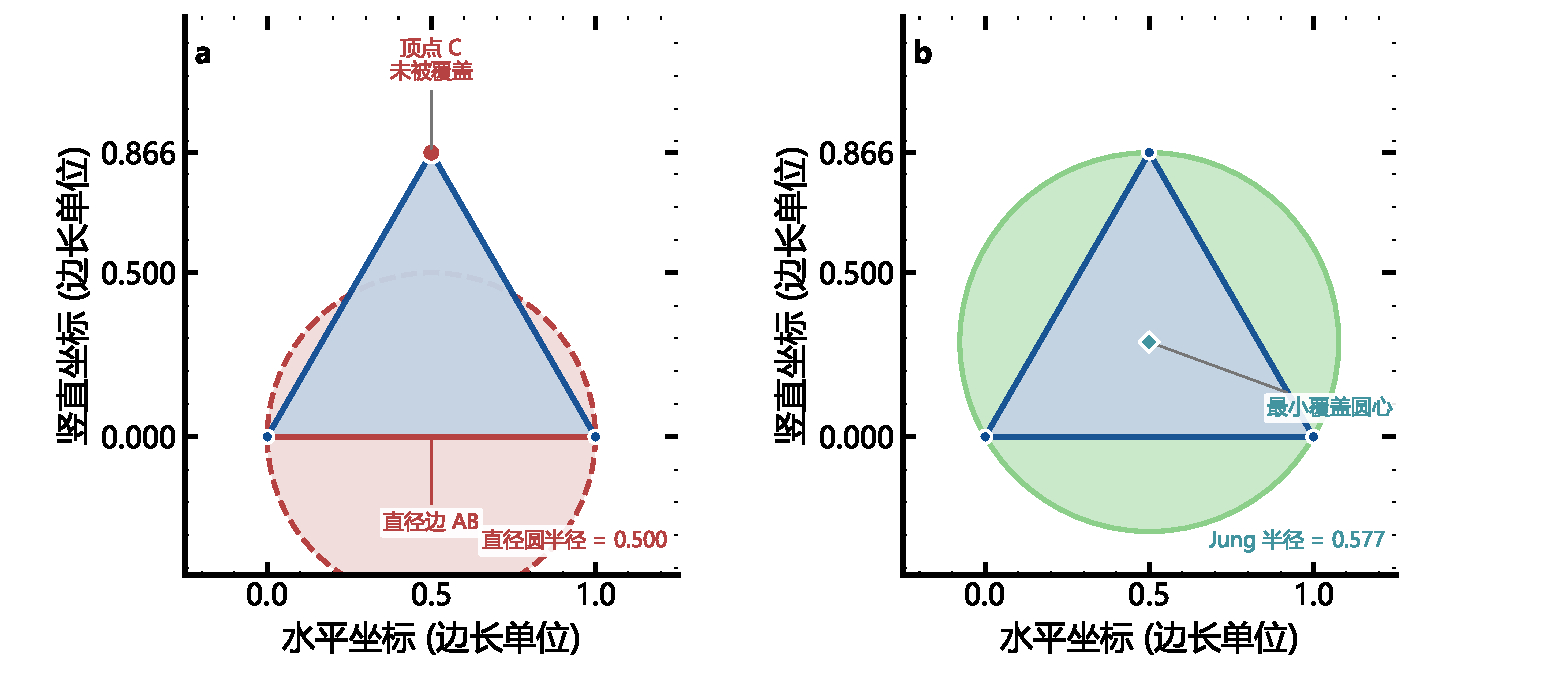
\includegraphics[width=0.92\textwidth]{figures/fig_q1_diameter.pdf}
\caption{等边三角形上，以最长边为直径的圆不能覆盖全部顶点（a）；Jung 最小覆盖圆半径约为边长的 $1/\sqrt{3}$（b）。演示数据来自 \texttt{q1\_q2\_demo.json}。}
\label{fig:q1_diameter}
\end{figure}

\begin{figure}[H]
\centering
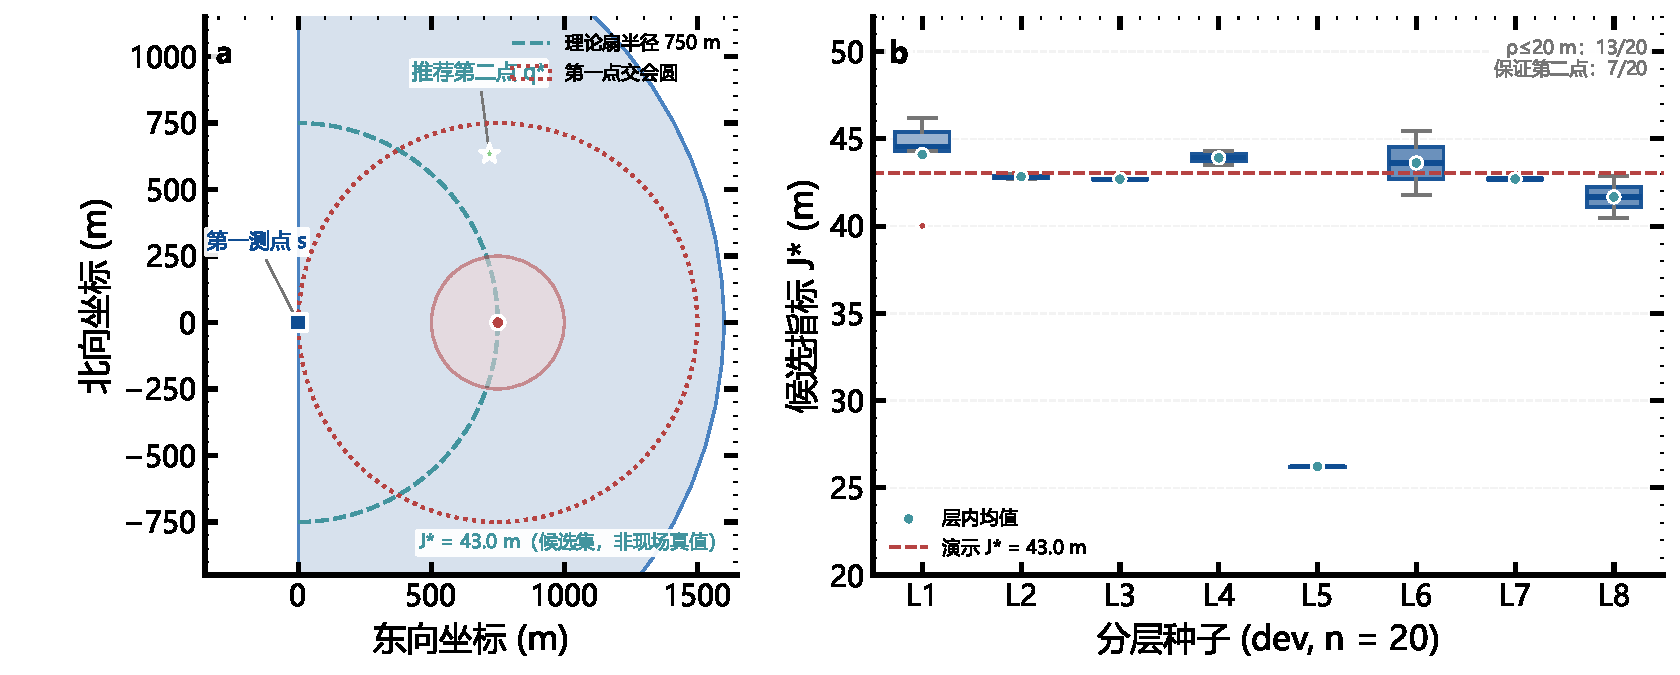
\includegraphics[width=0.95\textwidth]{figures/fig_q2_candidate.pdf}
\caption{问题2第二测点候选几何：前向 $180^\circ$ 扇、理论扇半径约 $750\,\mathrm{m}$ 与推荐点 $q^*$（a）；分层种子（dev，$n=20$）上候选指标 $J^*$ 的分布（b）。$J^*$ 仅为候选集推荐，非正式现场真值。}
\label{fig:q2_candidate}
\end{figure}

\begin{figure}[H]
\centering
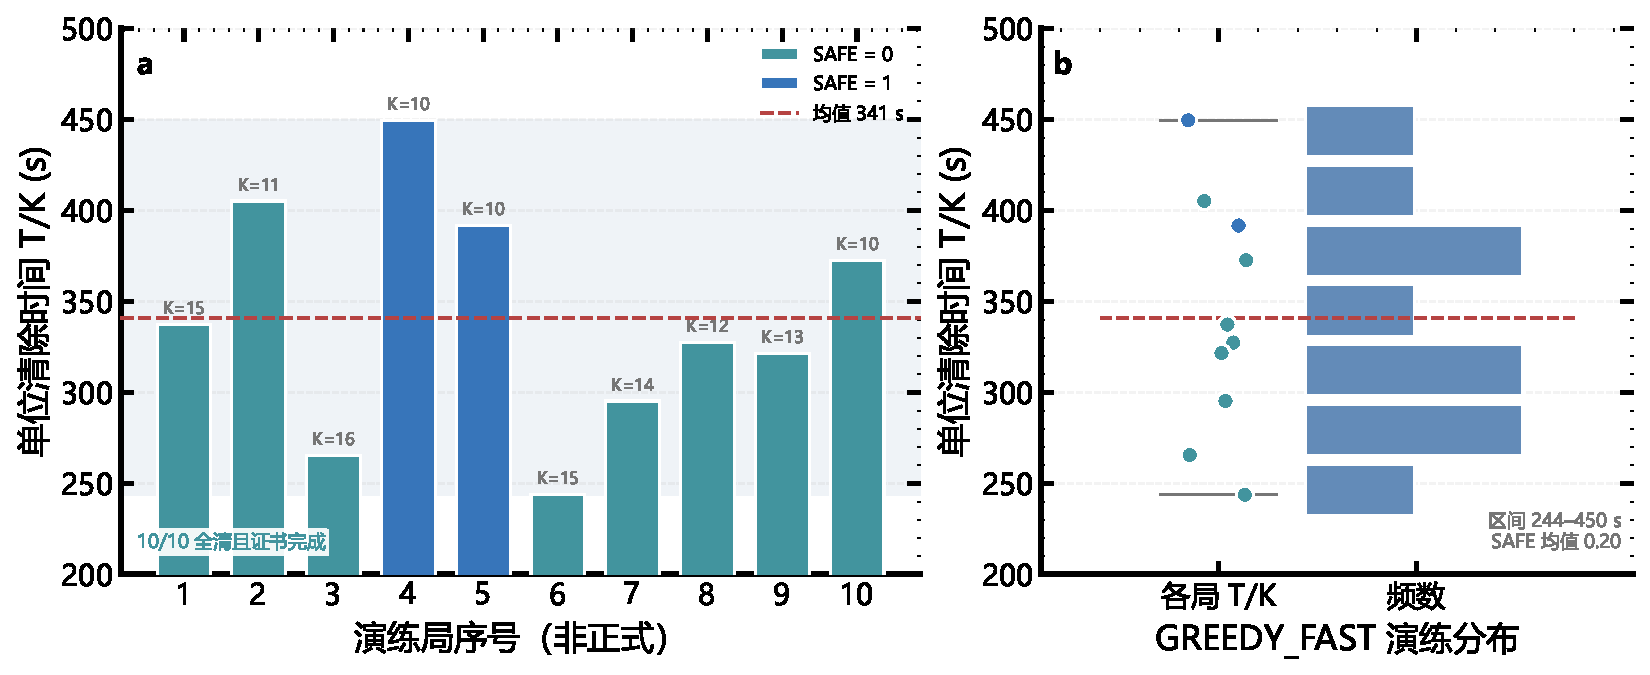
\includegraphics[width=0.95\textwidth]{figures/fig_q3_practice_tk.pdf}
\caption{GREEDY\_FAST 十局非正式演练的单位清除时间 $T/K$（a）及其分布（b）。$10/10$ 全清且证书完成，均值约 $341\,\mathrm{s}$。非正式、非配对，禁止填入表1正式成绩。}
\label{fig:q3_practice_tk}
\end{figure}

\begin{figure}[H]
\centering
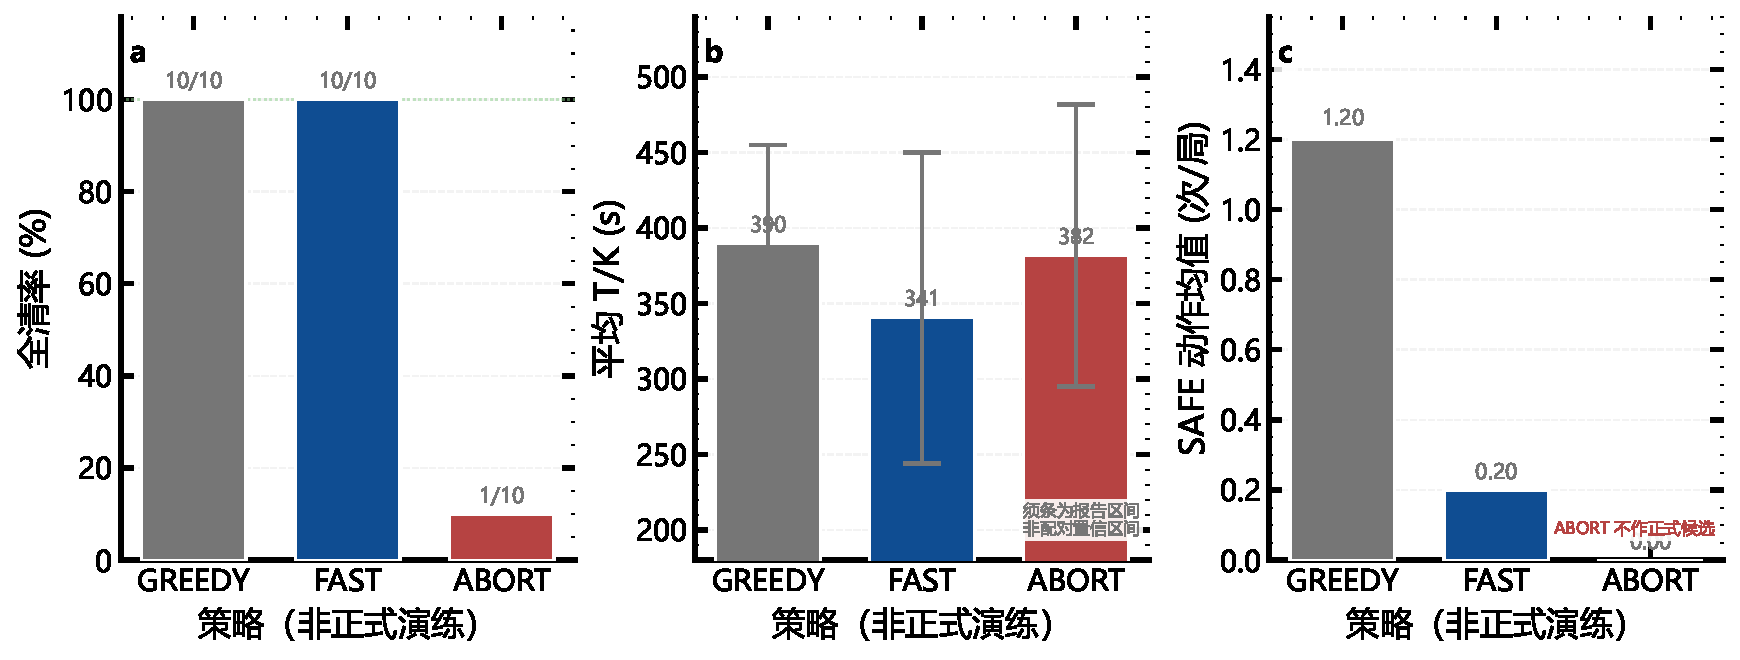
\includegraphics[width=0.95\textwidth]{figures/fig_q3_strategy.pdf}
\caption{问题3策略对照：全清率（a）、平均 $T/K$ 及报告区间（b）、SAFE 动作均值（c）。须条为已发表演练区间，非配对置信区间。GREEDY\_ABORT 不作正式候选。非正式、非配对。}
\label{fig:q3_strategy}
\end{figure}

\begin{figure}[H]
\centering
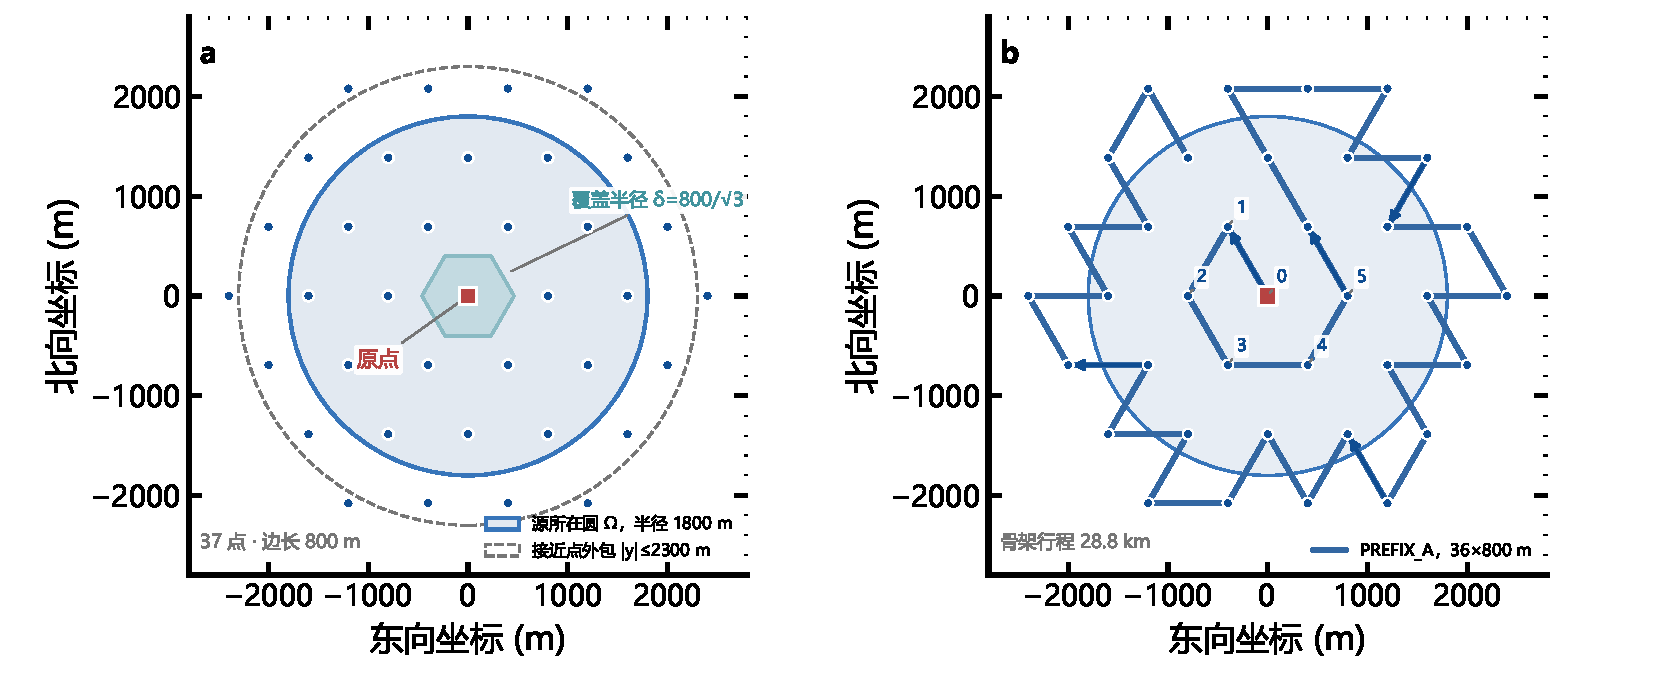
\includegraphics[width=0.95\textwidth]{figures/fig_q4_hex37.pdf}
\caption{HEX37 三角格点、源所在圆 $\Omega$（半径 $1800\,\mathrm{m}$）与覆盖半径 $\delta=800/\sqrt{3}$（a）；PREFIX\_A Hamilton 骨架（$36\times 800\,\mathrm{m}$，行程 $28.8\,\mathrm{km}$）（b）。}
\label{fig:q4_hex37}
\end{figure}

\begin{figure}[H]
\centering
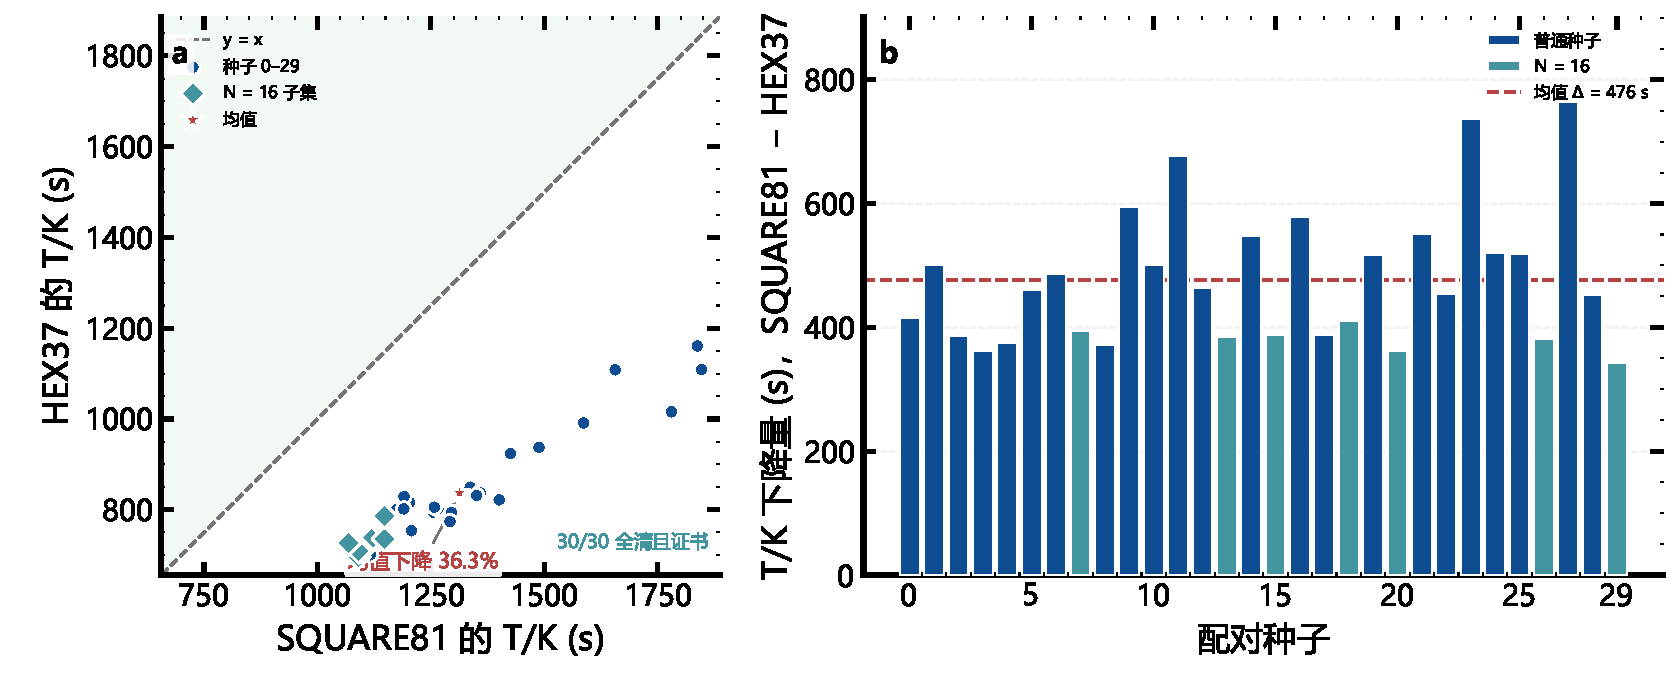
\includegraphics[width=0.95\textwidth]{figures/fig_q4_paired_tk.pdf}
\caption{配对种子 $0$--$29$ 上 SQUARE81 与 HEX37 的离线 $T/K$（a）及逐种子下降量（b）。双方 $30/30$ 全清且证书完成。离线几何模型，非正式。}
\label{fig:q4_paired_tk}
\end{figure}

\begin{figure}[H]
\centering
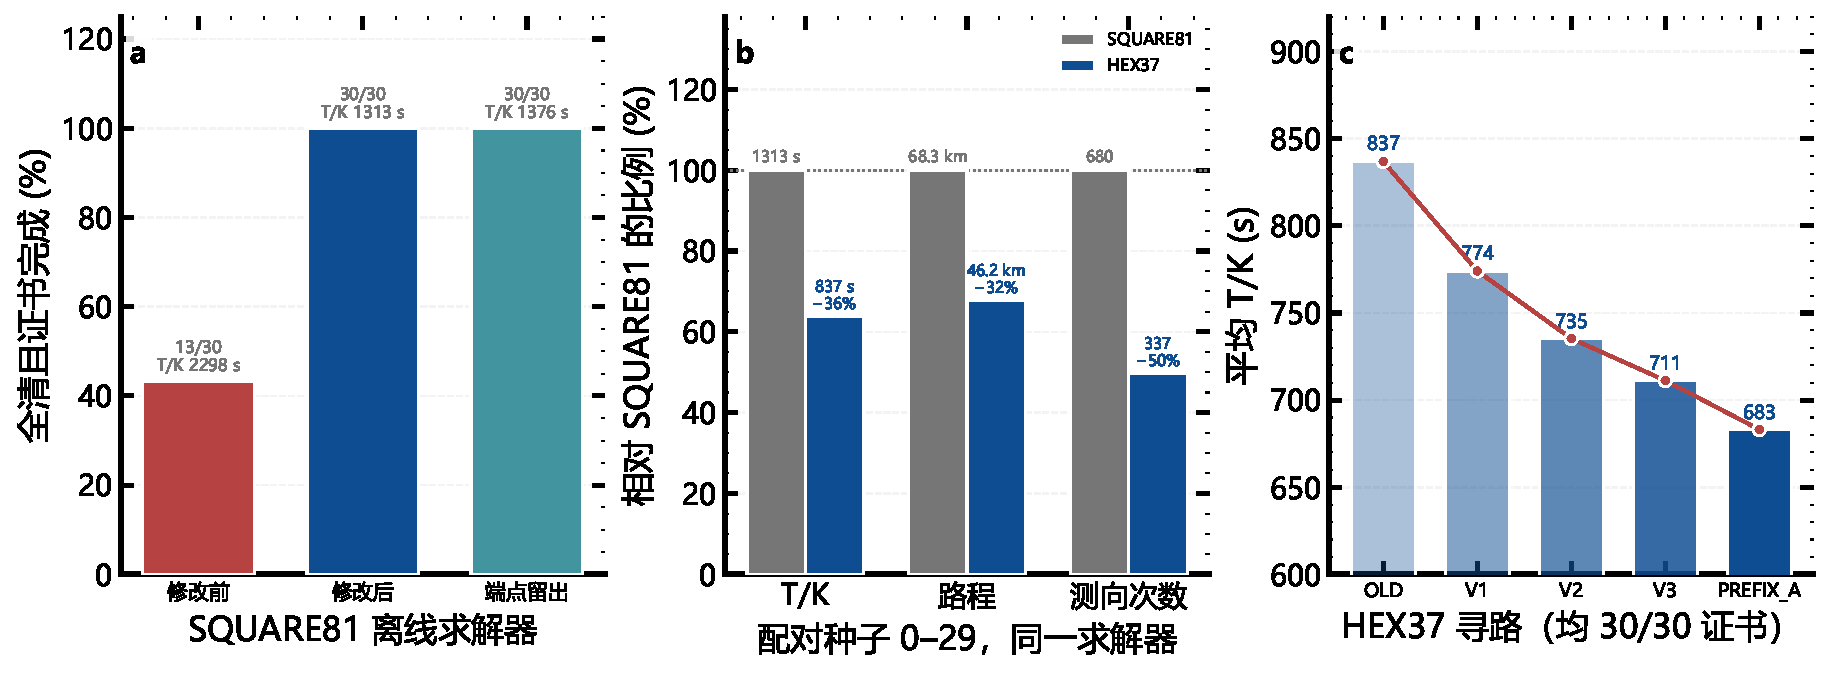
\includegraphics[width=0.98\textwidth]{figures/fig_q4_cover_compare.pdf}
\caption{SQUARE81 求解器修复前后与端点留出的全清率（a）；同一求解器下 HEX37 相对 SQUARE81 的 $T/K$、路程与测向次数（b）；HEX37 寻路 OLD$\to$PREFIX\_A 的平均 $T/K$（c）。离线几何模型；正式测试未执行。}
\label{fig:q4_cover_compare}
\end{figure}

% DrawIO 流程/架构图（源文件 .drawio；PDF 由 mxGraph 回退导出）
% 题注不超过 20 个汉字；keepaspectratio；非正式成绩不得入表1。

\begin{figure}[H]
\centering
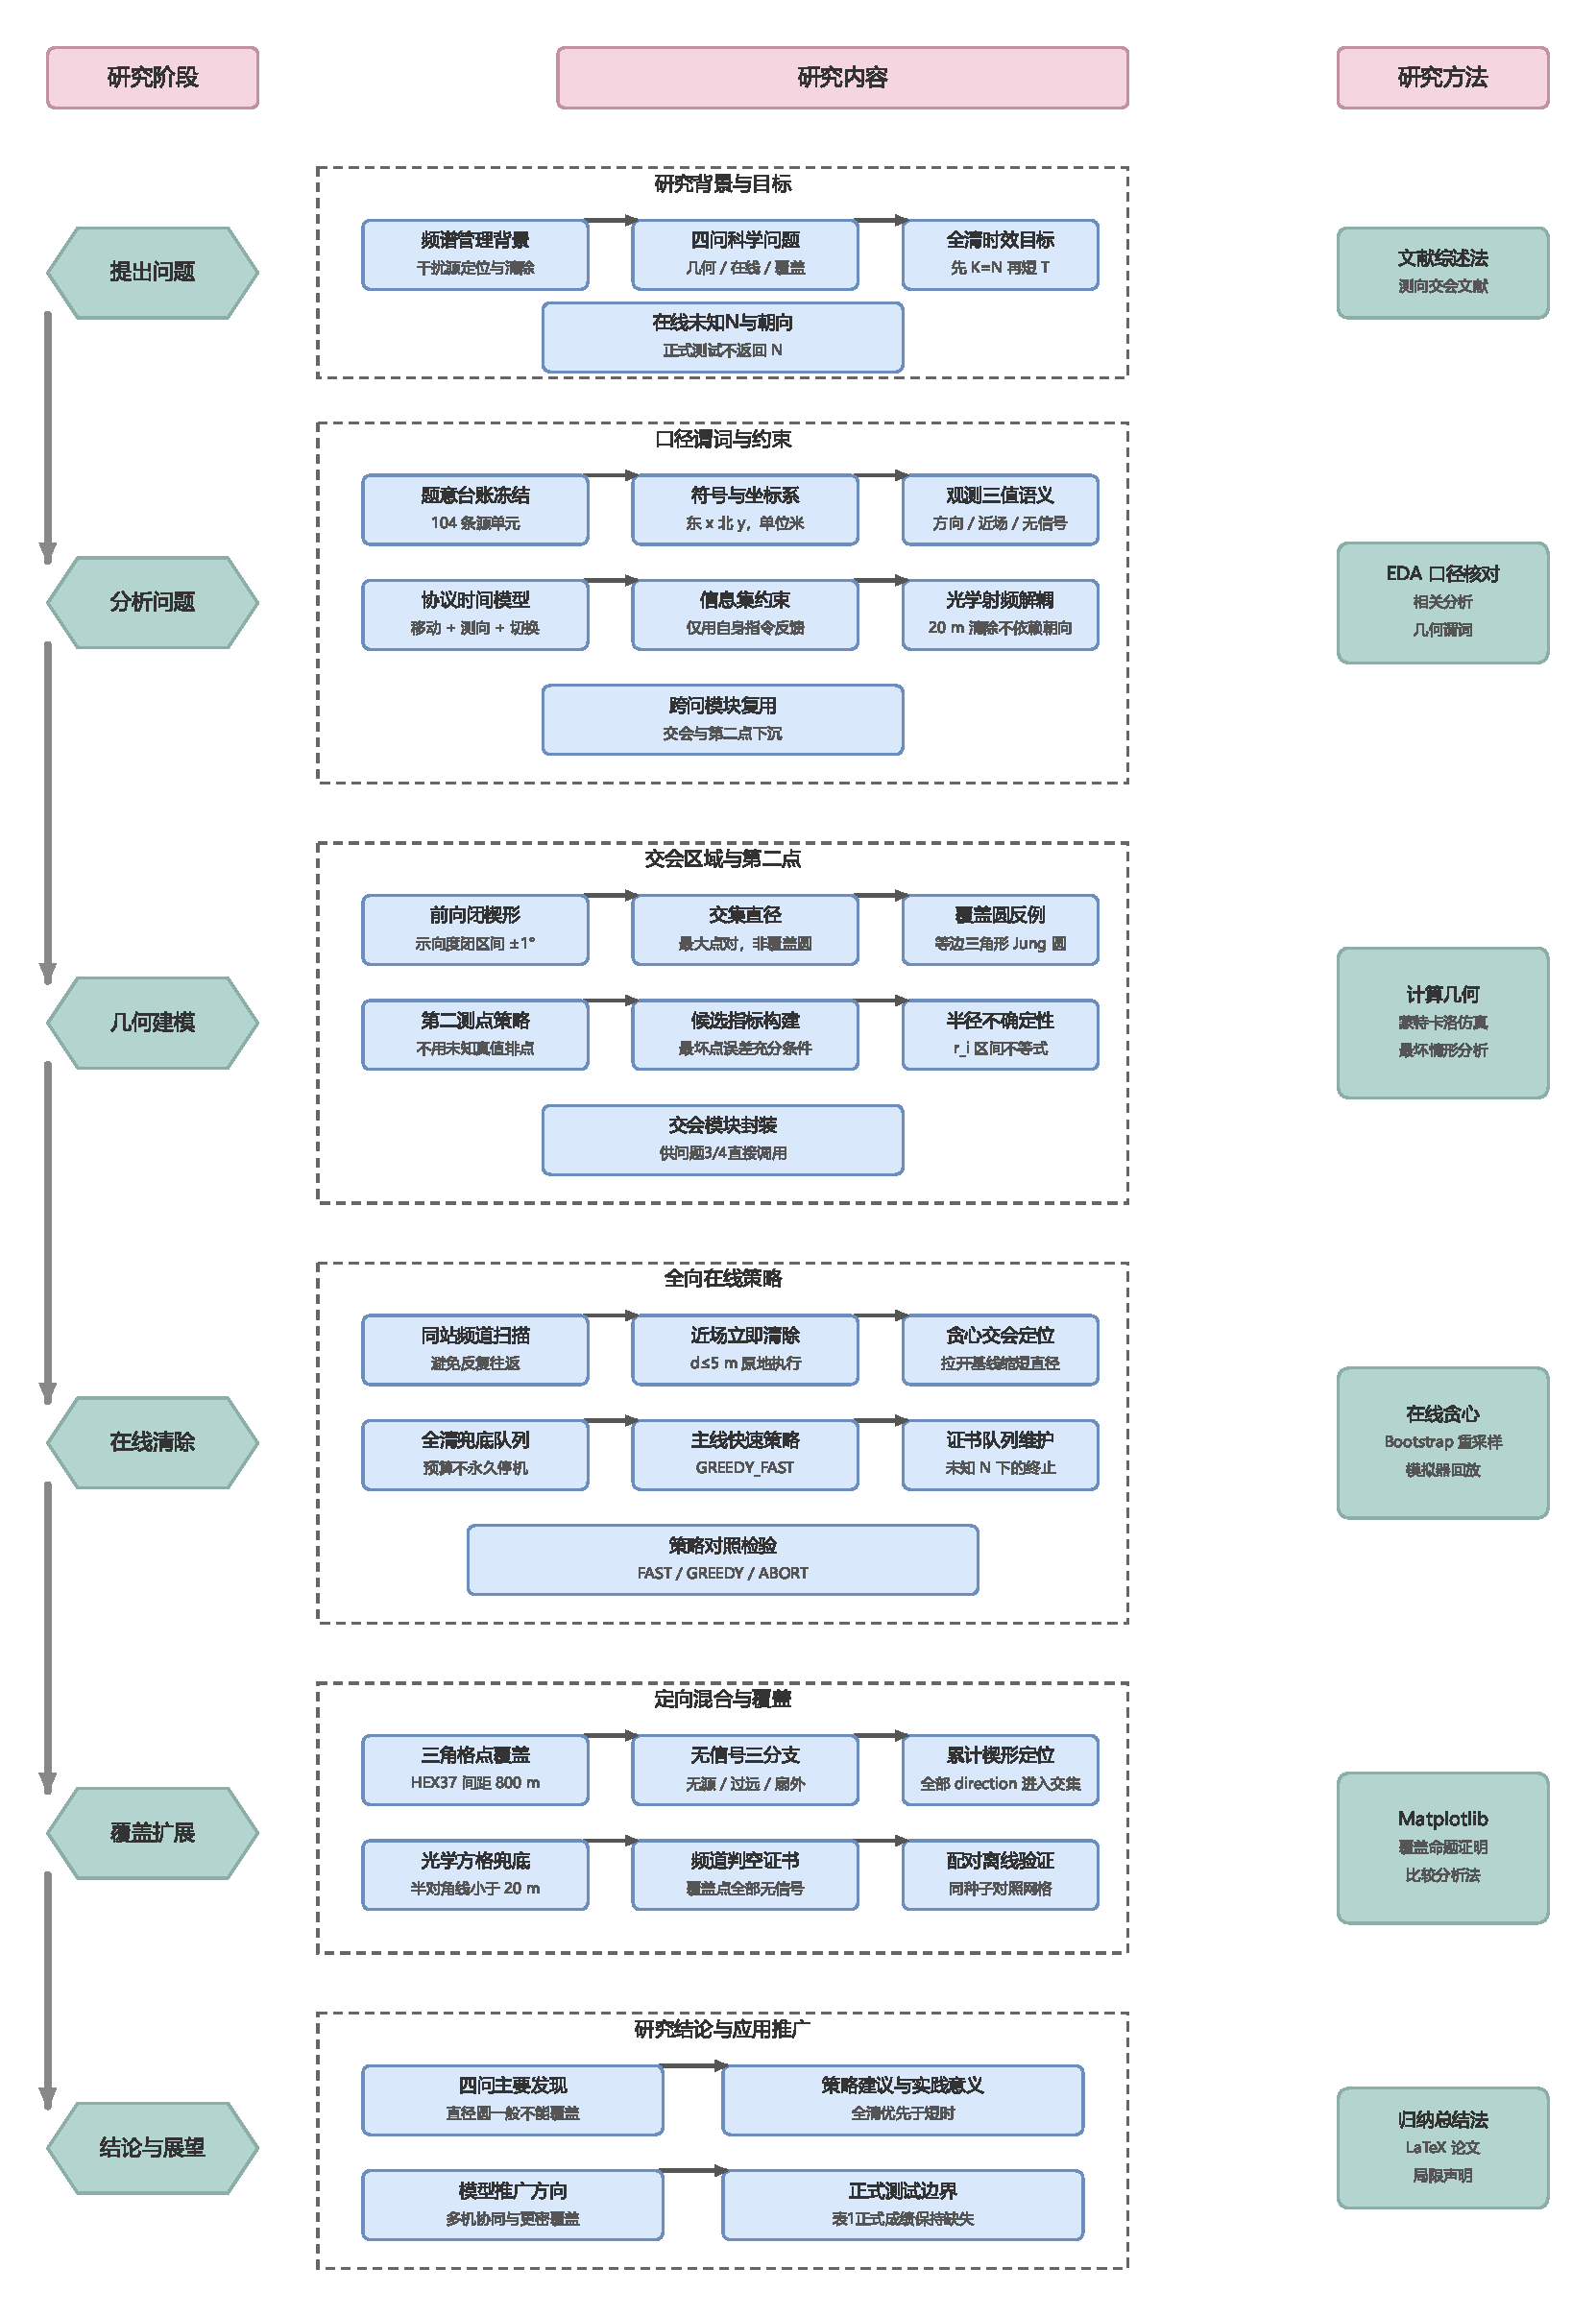
\includegraphics[width=0.85\textwidth,height=0.7\textheight,keepaspectratio]{figures/fig_roadmap.pdf}
\caption{技术路线总览}
\label{fig:roadmap}
\end{figure}

\begin{figure}[H]
\centering
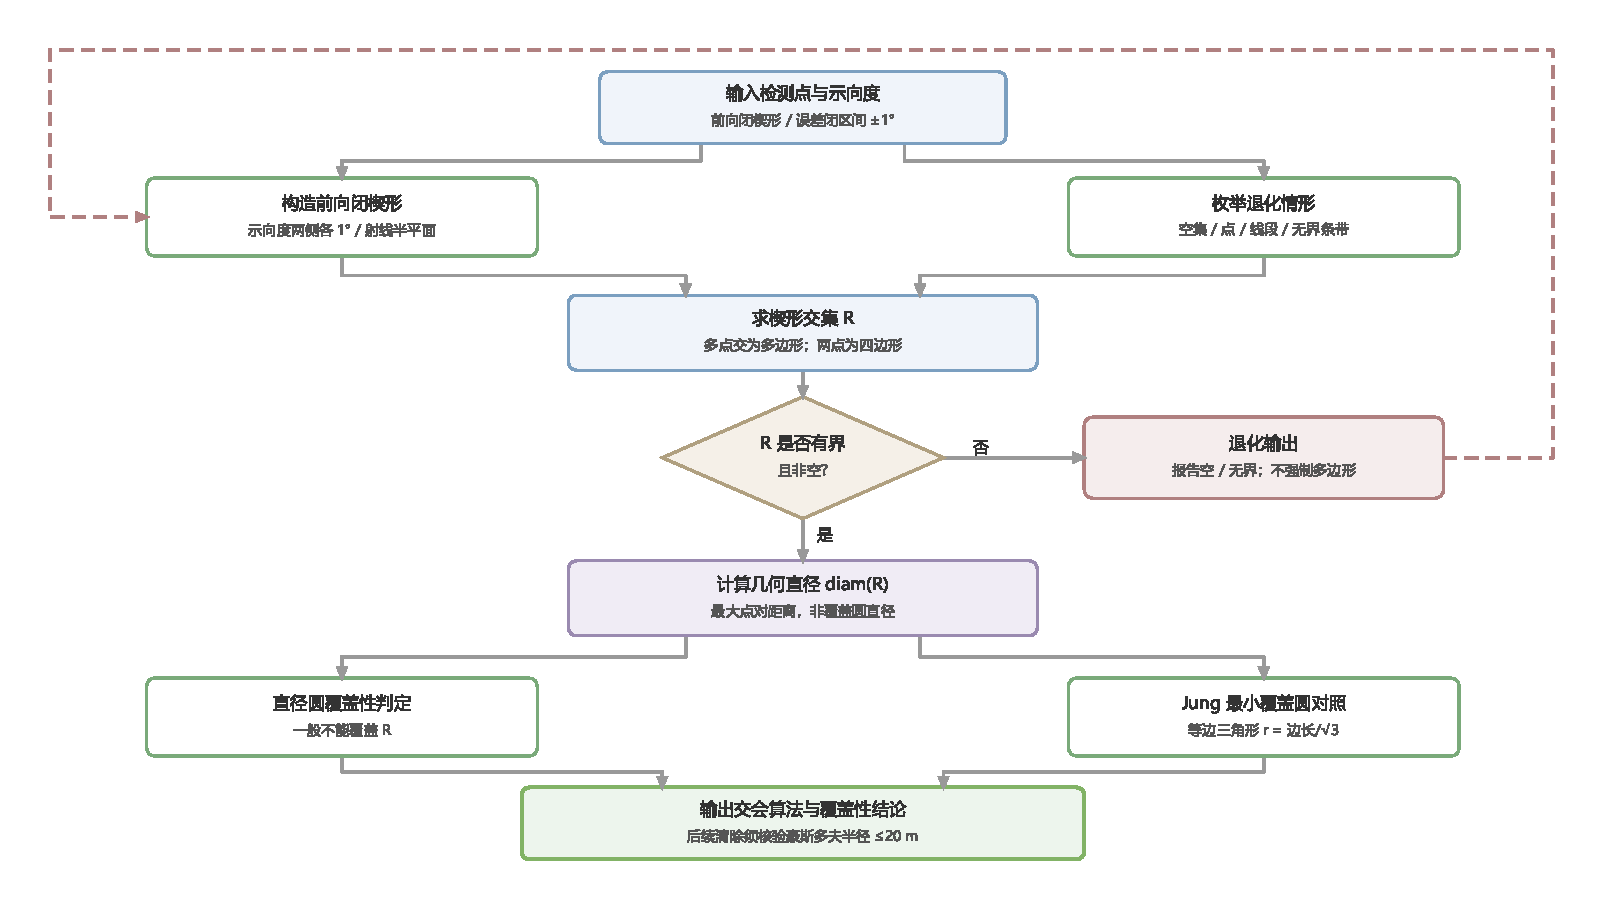
\includegraphics[width=0.82\textwidth,height=0.55\textheight,keepaspectratio]{figures/fig_flow_q1.pdf}
\caption{问题1交会求解流程}
\label{fig:flow_q1}
\end{figure}

\begin{figure}[H]
\centering
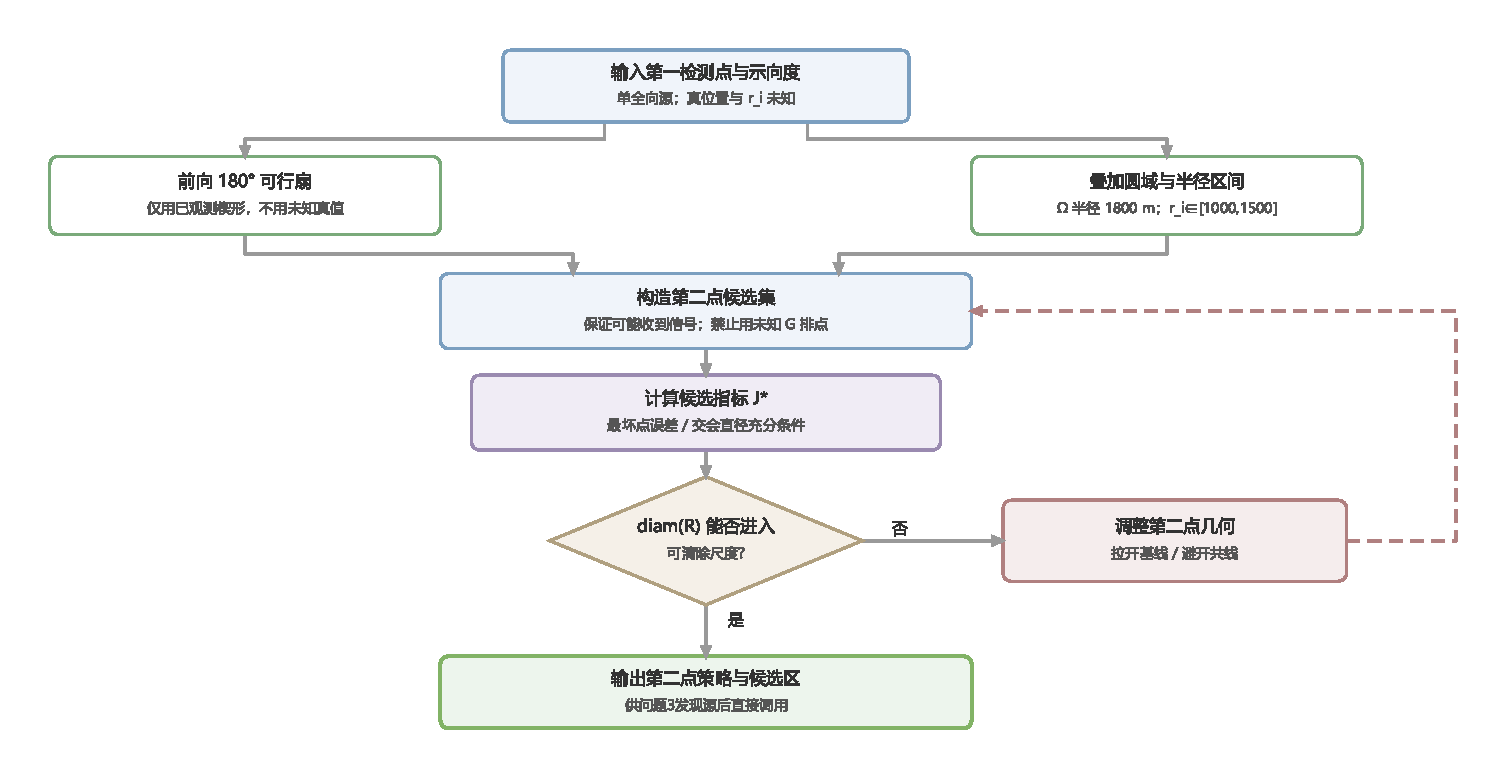
\includegraphics[width=0.82\textwidth,height=0.55\textheight,keepaspectratio]{figures/fig_flow_q2.pdf}
\caption{问题2第二点求解流程}
\label{fig:flow_q2}
\end{figure}

\begin{figure}[H]
\centering
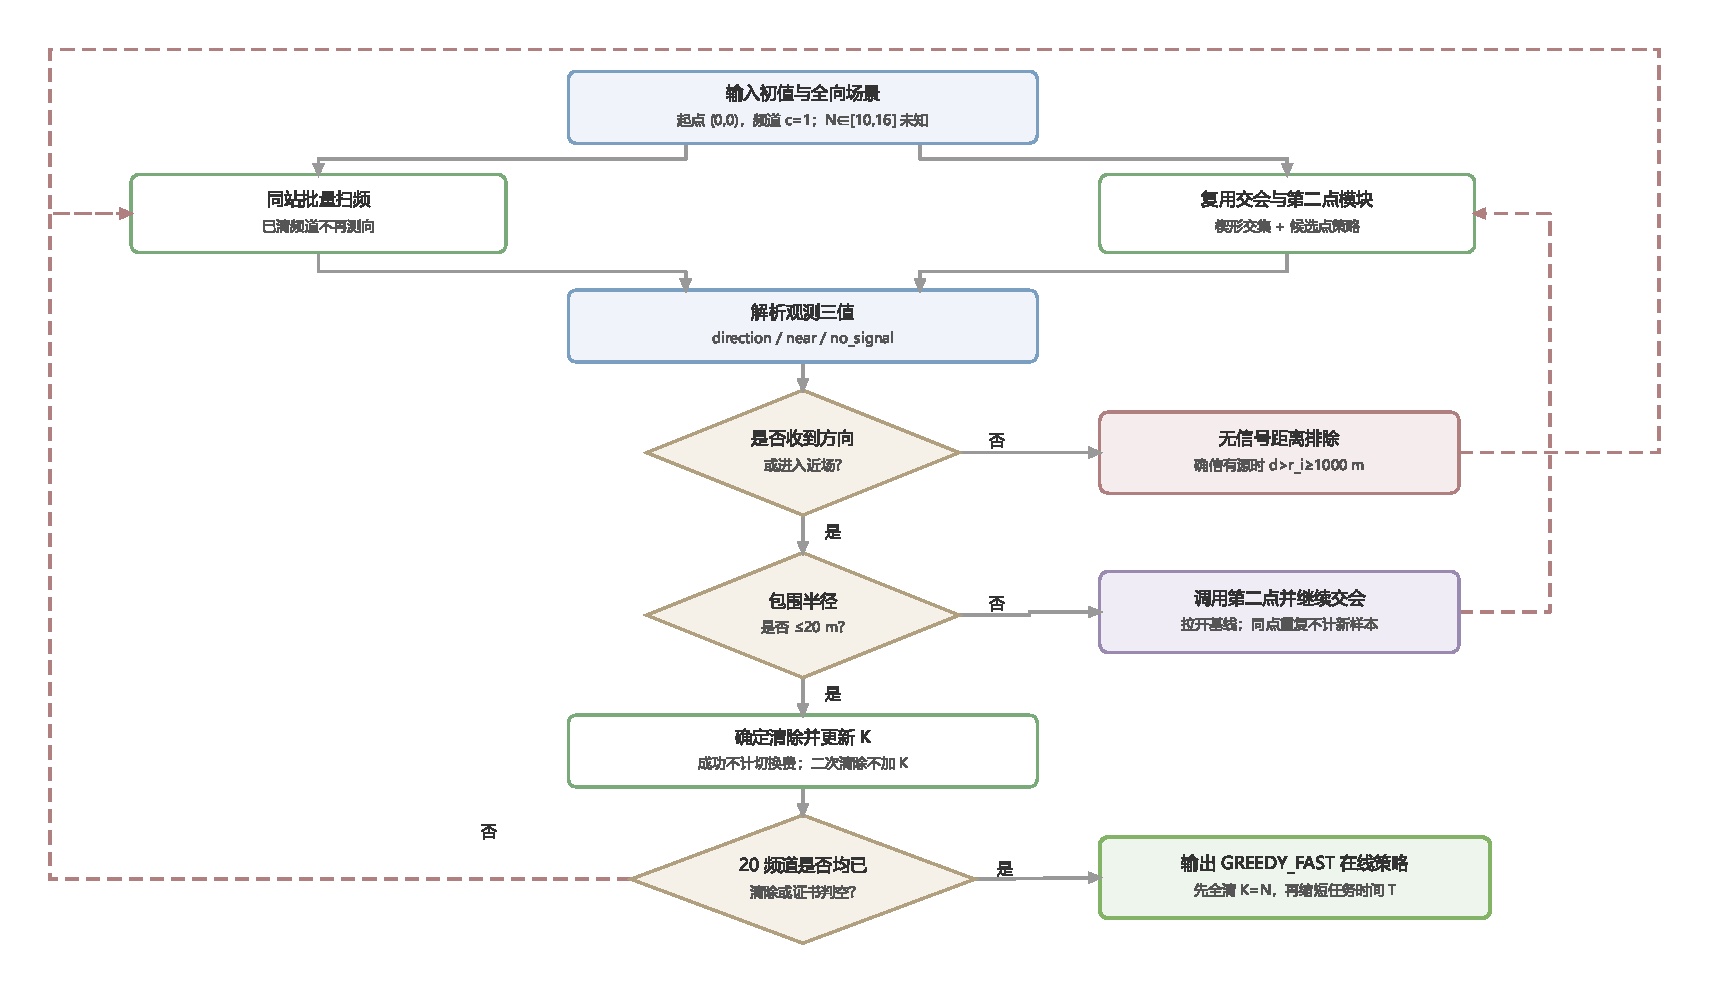
\includegraphics[width=0.82\textwidth,height=0.55\textheight,keepaspectratio]{figures/fig_flow_q3.pdf}
\caption{问题3在线清除流程}
\label{fig:flow_q3}
\end{figure}

\begin{figure}[H]
\centering
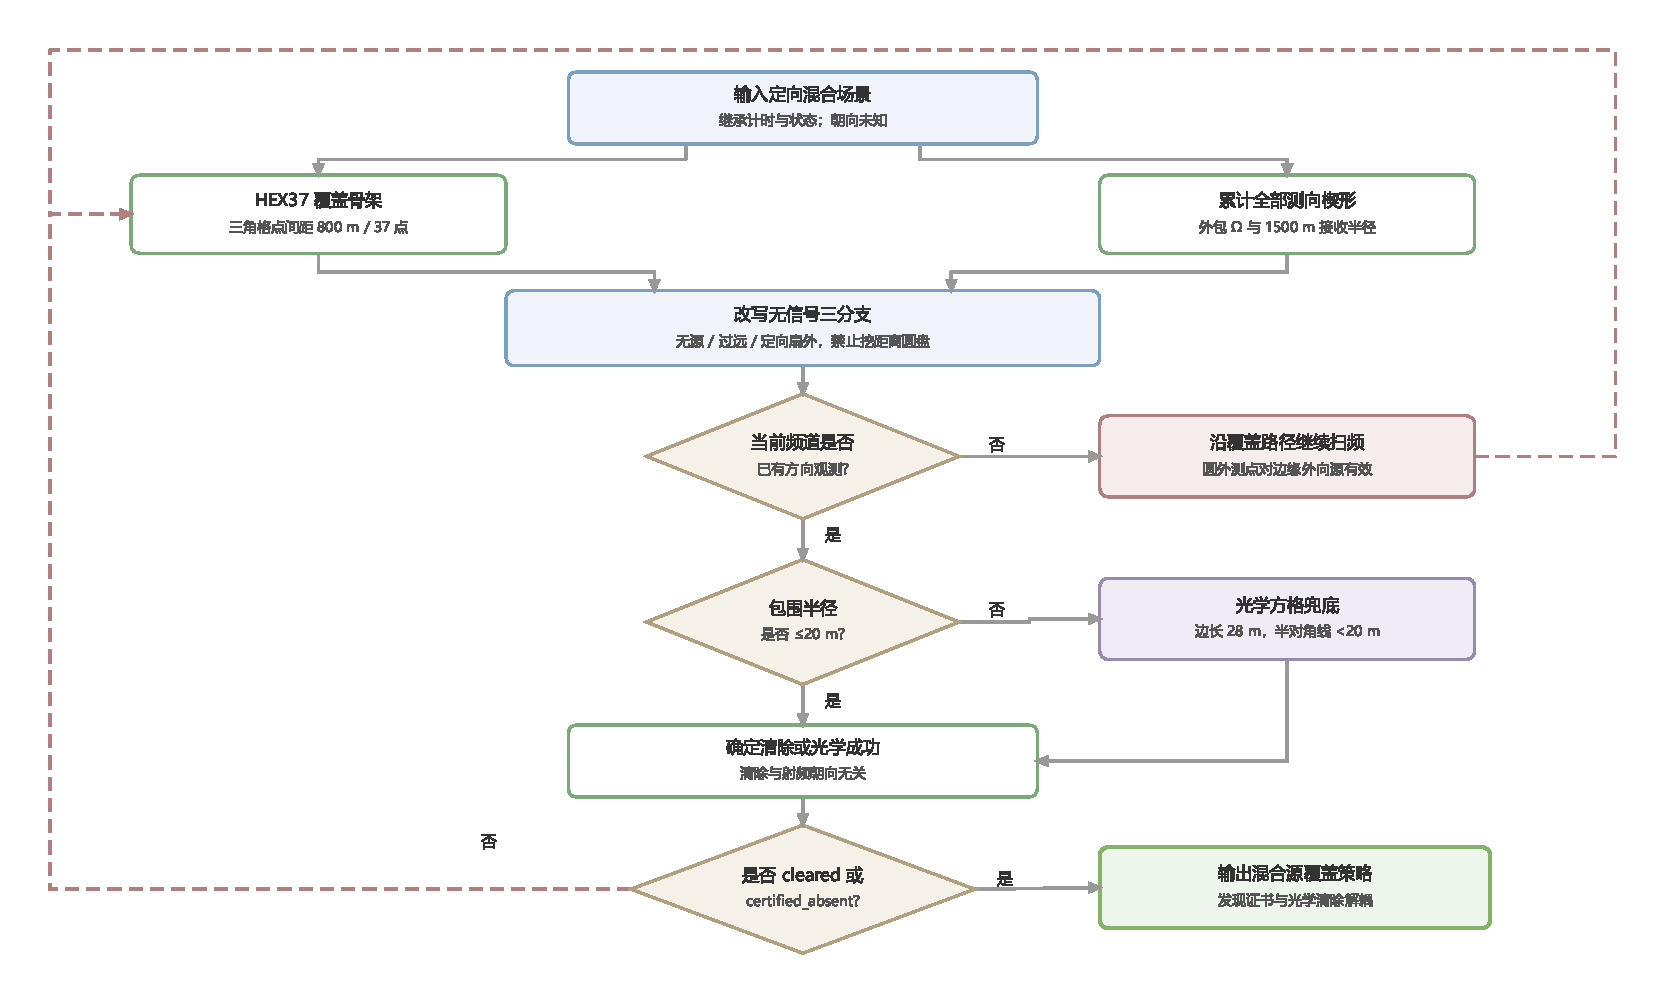
\includegraphics[width=0.82\textwidth,height=0.55\textheight,keepaspectratio]{figures/fig_flow_q4.pdf}
\caption{问题4混合源覆盖流程}
\label{fig:flow_q4}
\end{figure}

% TikZ 几何示意图（standalone XeLaTeX）

\begin{figure}[H]
\centering
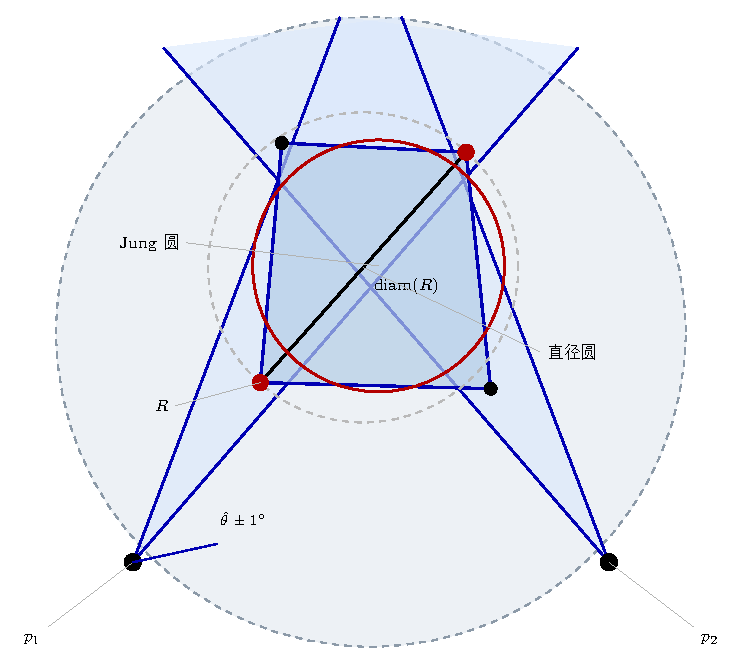
\includegraphics[width=0.82\textwidth,keepaspectratio]{figures/tikz_wedge_q1.pdf}
\caption{楔形交会与覆盖圆}
\label{fig:tikz_wedge_q1}
\end{figure}

\begin{figure}[H]
\centering
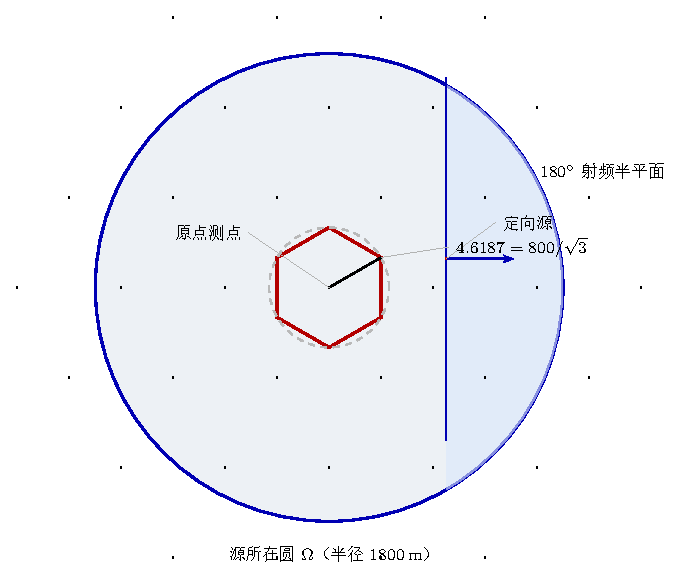
\includegraphics[width=0.82\textwidth,keepaspectratio]{figures/tikz_hex37_cover.pdf}
\caption{HEX37覆盖与定向扇}
\label{fig:tikz_hex37_cover}
\end{figure}
